\section{Code protection scheme of \DSVMP}\label{sec:overview}
To address the problem of cumulative attacks, we want to introduce a certain
degree of diversity and uncertainty into program execution. This is achieved
through using a diversified scheduling structure (Section~\ref {sec:dvs}) and
multiple VMs (Section~\ref {sec:mvm}) in \DSVMP. Like other VM-based protection schemes,
\DSVMP focuses on protecting critical code regions to minimize the runtime overhead.
Figure~\ref{fig:Fig.2} depicts the system architecture of \DSVMP.
Code protection of \DSVMP follows several steps described as follows:

\begin{figure}[!t]
  \centering
  % Requires \usepackage{graphicx}
  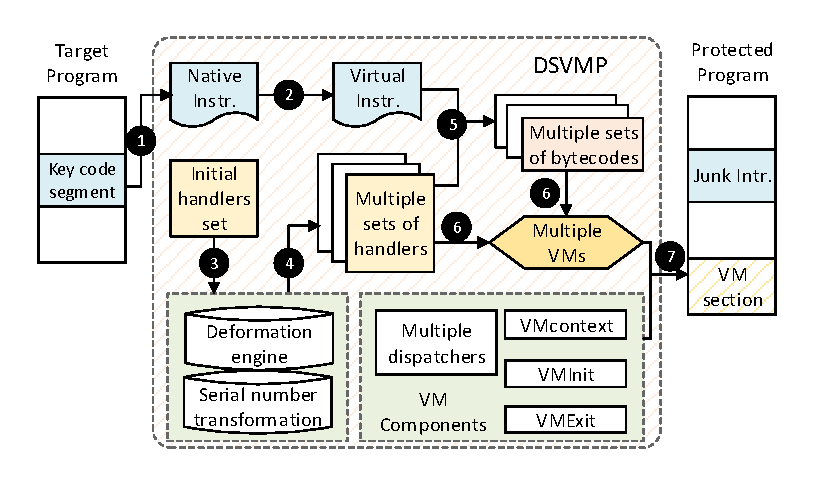
\includegraphics[width=0.7\columnwidth]{figure/figtwo.pdf}
  \caption{Offline code protection process. \DSVMP takes in a program binary. For each protected code region, it translates native instructions into bytecodes. Next, it generates multiple bytecode handlers that are semantically equivalent but implemented in different ways. It then generates the corresponding driver-data and multiple VMs. Finally, the generated VMs and associated components will be inserted into the program binary and fills the original code region with junk instructions.}\label{fig:Fig.2}
  %\vspace{-5mm}
\end{figure}

\paragraph*{Code translation}
\DSVMP takes in a compiled program binary and does not require having access to the source code.
Code segments need to be protected are translated into native machine instructions (e.g. x86 instructions)
using a disassembler (Step \ding{182}), which will then be mapped into a set of virtual instructions (Step \ding{183}).

\paragraph*{Diversifying}
As a departure from prior work on VM-based code obfuscation, \DSVMP employs multiple VM instruction scheduling policies
where each scheduler can have more than one dispatcher and one handler can be scheduled by another handler
and each virtual instructions can be interpreted by more than one handlers.
A set of initial handlers will be randomly obfuscated to provide stronger protection for the particular code region (Step \ding{184}).
Furthermore, each handler will be obfuscated $VMNum$ ($VMNum >= 1$) times by using the deformation engine, resulting in $VMNum$ sets of semantically equivalent handlers with different implementations and control flows (Step \ding{185}). Then, virtual instructions are encoded into $2*VMNum$ sets of bytecodes. For each set of handlers, there will be two sets of corresponding bytecodes (details in Section~\ref {sec:mbd}) (Step \ding{186}). Subsequently, \DSVMP constructs multiple VMs, where each VM contains one set of handlers and two sets of bytecodes (Step \ding{187}).

\paragraph*{Code generation}
Finally, a new section will be inserted into the program binary, which contains $VMNum$ VMs and their components such as dispatchers, VMContext etc. It also fills the original code region with junk instructions (Step \ding{188}).

This is an overview of our approach. We describe the implementation of \DSVMP in more details in the following sections.
